\part{Lecture 03: Dynamic Programming}
\title[RL Lecture 03]{Lecture 03: Dynamic Programming}  
\date{}  
\frame{\titlepage} 
\frame{\frametitle{Table of Contents}\tableofcontents} 

%%%%%%%%%%%%%%%%%%%%%%%%%%%%%%%%%%%%%%%%%%%%%%%%%%%%%%%%%%%%%%%%%%
\section{Introduction} 
%%%%%%%%%%%%%%%%%%%%%%%%%%%%%%%%%%%%%%%%%%%%%%%%%%%%%%%%%%%%%%%%%%

%%%%%%%%%%%%%%%%%%%%%%%%%%%%%%%%%%%%%%%%%%%%%%%%%%%%%%%%%%%%%
%% What is Dynamic Programming? %%
%%%%%%%%%%%%%%%%%%%%%%%%%%%%%%%%%%%%%%%%%%%%%%%%%%%%%%%%%%%%%
\frame{\frametitle{What is Dynamic Programming (DP)?}

\begin{block}{Basic DP definition}
\begin{itemize}
	\item \hl{Dynamic}: sequential or temporal problem structure
	\item \hl{Programming}: mathematical optimization, i.e., numerical solutions
\end{itemize}
\end{block}
\pause
\vspace{1cm}
Further characteristics:
\begin{itemize}
	\item DP is a collection of algorithms to solve MDPs and neighboring problems.
	\begin{itemize}
		\item \hl{We will focus only on finite MDPs.}
		\item In case of continuous action/state space: apply quantization.
	\end{itemize}\pause
	\item Use of value functions to organize and structure the search for an optimal policy.
	\item Breaks problems into subproblems and solves them.
\end{itemize}
}

%%%%%%%%%%%%%%%%%%%%%%%%%%%%%%%%%%%%%%%%%%%%%%%%%%%%%%%%%%%%%
%% Requirements %%
%%%%%%%%%%%%%%%%%%%%%%%%%%%%%%%%%%%%%%%%%%%%%%%%%%%%%%%%%%%%%
\frame{\frametitle{Requirements for DP}
DP can be applied to problems with the following characteristics.
\begin{itemize}
	\item Optimal substructure:
	\begin{itemize}
		\item Principle of optimality applies.
		\item Optimal solution can be derived from subproblems.
	\end{itemize}\pause
\end{itemize}
\begin{itemize}
	\item Overlapping subproblems:
	\begin{itemize}
		\item Subproblems recur many times.
		\item Hence, solutions can be cached and reused.
	\end{itemize}
\end{itemize}\pause
\vspace{1cm}
How is that connected to MDPs?
\begin{itemize}
	\item MDPs satisfy above's properties:
	\begin{itemize}
		\item Bellman equation provides recursive decomposition.
		\item Value function stores and reuses solutions.
	\end{itemize}
\end{itemize}
}

%%%%%%%%%%%%%%%%%%%%%%%%%%%%%%%%%%%%%%%%%%%%%%%%%%%%%%%%%%%%%
%% Example: DP vs. Exhaustive Search (1)%%
%%%%%%%%%%%%%%%%%%%%%%%%%%%%%%%%%%%%%%%%%%%%%%%%%%%%%%%%%%%%%
\frame{\frametitle{Example: DP vs. Exhaustive Search (1)}
\begin{figure}		
	\animategraphics[loop,controls,width=10cm]{0.75}{fig/lec03/gif/PB_Bi_ES-}{0}{6}
	\caption{Shortest path problem to travel from Paderborn to Bielefeld: Eshaustive search requires 14 travel segment evaluations since every possible travel route is evaluated independently.}
	\label{fig:PB_Bi_ES}
\end{figure}
}

%%%%%%%%%%%%%%%%%%%%%%%%%%%%%%%%%%%%%%%%%%%%%%%%%%%%%%%%%%%%%
%% Example: DP vs. Exhaustive Search (2)%%
%%%%%%%%%%%%%%%%%%%%%%%%%%%%%%%%%%%%%%%%%%%%%%%%%%%%%%%%%%%%%
\frame{\frametitle{Example: DP vs. Exhaustive Search (2)}
\begin{figure}		
	\animategraphics[loop,controls,width=10cm]{0.75}{fig/lec03/gif/PB_Bi_DP-}{0}{5}
	\caption{Shortest path problem to travel from Paderborn to Bielefeld: DP requires only 10 travel segment evaluations in order to calculate the optimal travel policy due to the reuse of subproblem results.}
	\label{fig:PB_Bi_DP}
\end{figure}
}

%%%%%%%%%%%%%%%%%%%%%%%%%%%%%%%%%%%%%%%%%%%%%%%%%%%%%%%%%%%%%
%% Utility DP %%
%%%%%%%%%%%%%%%%%%%%%%%%%%%%%%%%%%%%%%%%%%%%%%%%%%%%%%%%%%%%%
\frame{\frametitle{Utility of DP in the RL Context}
DP is used for iterative \hl{planning} (i.e., \hl{model-based} prediction and control) in an MDP.
\begin{itemize}
	\item Prediction:
	\begin{itemize}
		\item Input: MDP $\left\langle\mathcal{X}, \mathcal{U}, \bm{\mathcal{P}}, \mathcal{R}, \gamma \right\rangle$ and policy $\pi$
		\item Output: (estimated) value function $\hat{v}_{\pi} \approx v_{\pi}$
	\end{itemize}\pause
	\item Control:
	\begin{itemize}
		\item Input: MDP $\left\langle\mathcal{X}, \mathcal{U}, \bm{\mathcal{P}}, \mathcal{R}, \gamma \right\rangle$
		\item Output: (estimated) optimal value function $\hat{v}_{\pi}^* \approx v_{\pi}^*$ or policy $\hat{\pi}^*\approx\pi^*$
	\end{itemize}\pause
\end{itemize}
\vspace{1cm}
In both applications \hl{DP requires full knowledge of the MDP} structure.
\begin{itemize}
	\item Feasibility in real-world engineering applications (model vs. system) is therefore limited.\pause
	\item But: \hl{following DP concepts are largely used in modern data-driven RL algorithms.}
\end{itemize}
}

%%%%%%%%%%%%%%%%%%%%%%%%%%%%%%%%%%%%%%%%%%%%%%%%%%%%%%%%%%%%%%%%%%
\section{Policy Evaluation} 
%%%%%%%%%%%%%%%%%%%%%%%%%%%%%%%%%%%%%%%%%%%%%%%%%%%%%%%%%%%%%%%%%%
\begin{frame}
\frametitle{Table of Contents}
\tableofcontents[currentsection]
\end{frame}

%%%%%%%%%%%%%%%%%%%%%%%%%%%%%%%%%%%%%%%%%%%%%%%%%%%%%%%%%%%%%
%% Policy Evaluation Background (1) %%
%%%%%%%%%%%%%%%%%%%%%%%%%%%%%%%%%%%%%%%%%%%%%%%%%%%%%%%%%%%%%
\frame{\frametitle{Policy Evaluation Background (1)}
\begin{itemize}
	\item Problem: evaluate a given policy $\pi$ to predict $v_\pi$. \pause
	\item Recap: Bellman equation for $x_k\in\mathcal{X}$ is given as
	\begin{align*}
	v_\pi(x_k) &= \El{G_k|X_k=x_k}{\pi},\\
									&= \El{R_{k+1}+ \gamma G_{k+1}|X_k=x_k}{\pi},\\
									&= \El{R_{k+1}+ \gamma v_\pi(X_{k+1})|X_k=x_k}{\pi}.
	\end{align*}\vspace{-0.5cm}\pause
	\item Or in matrix form:
		\begin{equation*}
			\begin{split}
					\bm{v}_{\mathcal{X}}^{\pi}&=\bm{r}_{\mathcal{X}}^{\pi}+\gamma\bm{\mathcal{P}}_{xx'}^{\pi}\bm{v}_{\mathcal{X}}^{\pi},\\
					\begin{bmatrix} v_{1}^{\pi} \\ \vdots \\ v_{n}^{\pi} \end{bmatrix} &= \begin{bmatrix} \mathcal{R}_{1}^{\pi} \\ \vdots \\ \mathcal{R}_{n}^{\pi} \end{bmatrix} + \gamma\begin{bmatrix} p_{11}^{\pi} & \cdots & p_{1n}^{\pi}\\ \vdots &  & \vdots\\ p_{n1}^{\pi} & \cdots & p_{nn}^{\pi}\end{bmatrix}\begin{bmatrix} v_{1}^{\pi} \\ 			\vdots \\ v_{n}^{\pi} \end{bmatrix}.
			\end{split}
			\end{equation*}\pause
			\item Solving the Bellman equation for $v_\pi$ requires handling a linear equation system with $n$ unknowns (i.e., number of states).
			\item Remember that the reward function $\mathcal{R}_{x}^{\pi}$ might also contains stochastic influences depending on the MDP structure (see \defref{defi:Markov_decision_process}).
\end{itemize}
}

%%%%%%%%%%%%%%%%%%%%%%%%%%%%%%%%%%%%%%%%%%%%%%%%%%%%%%%%%%%%%
%% Policy Evaluation Background (2) %%
%%%%%%%%%%%%%%%%%%%%%%%%%%%%%%%%%%%%%%%%%%%%%%%%%%%%%%%%%%%%%
\frame{\frametitle{Policy Evaluation Background (2)}
\begin{itemize}
	\item Problem: directly calculating $v_\pi$ is numerically costly for high-dimensional state spaces (e.g., by matrix inversion). \pause
	\item General idea: \hl{apply iterative approximations} $\hat{v}_{i}(x_{k})=v_{i}(x_{k})$ of $v_\pi(x_{k})$ with decreasing errors:
	\begin{equation}
	\left\|v_{i}(x_{k}) - v_\pi\right\|_{\infty}\rightarrow 0 \quad \mbox{for} \quad i=1,2,3,\ldots
\end{equation}\pause
	\item The Bellman equation in matrix form can be rewritten as:
	\begin{equation}
	\label{eq:Bellman_matrix_Ab}
	\underbrace{\left(\bm{I}-\gamma\bm{\mathcal{P}}_{xx'}^{\pi}\right)}_{\bm{A}}\underbrace{\bm{v}_{\mathcal{X}}^{\pi}}_{\bm{\zeta}} =\underbrace{\bm{r}_{\mathcal{X}}^{\pi}}_{\bm{b}}.
\end{equation}\pause
\item To iteratively solve this linear equation $\bm{A}\bm{\zeta}=\bm{b}$, one can apply numerous methods such as
\begin{itemize}
	\item General gradient descent,
	\item Richardson iteration,
	\item Kyrlov subspace methods.
\end{itemize}
\end{itemize}
}

%%%%%%%%%%%%%%%%%%%%%%%%%%%%%%%%%%%%%%%%%%%%%%%%%%%%%%%%%%%%%
%% Richardson Iteration (1)%%
%%%%%%%%%%%%%%%%%%%%%%%%%%%%%%%%%%%%%%%%%%%%%%%%%%%%%%%%%%%%%
\frame{\frametitle{Richardson Iteration (1)}
In the MDP context, the Richardson iteration became the default solution approach to iteratively solve:
\begin{equation*}
	\bm{A}\bm{\zeta} =\bm{b}.
\end{equation*}
The \hl{Richardson iteration} is 
\begin{equation}
\label{eq:richardson_general}
	\bm{\zeta}_{i+1}= \bm{\zeta}_{i} + \omega(\bm{b}-\bm{A}\bm{\zeta}_i)
\end{equation}
with $\omega$ being a scalar parameter that has to be chosen such that the sequence $\bm{\zeta}_{i}$ converges. \pause To choose $\omega$ we inspect the series of approximation errors $\bm{e}_i=\bm{\zeta}_{i}-\bm{\zeta}$ and apply it to \eqref{eq:richardson_general}:
\begin{equation}
	\bm{e}_{i+1}= \bm{e}_{i} - \omega\bm{A}\bm{e}_i=\left(\bm{I}-\omega\bm{A}\right)\bm{e}_{i}.
\end{equation}\pause
To evaluate convergence we inspect the following norm:
\begin{equation}
\label{eq:richardson_error_sequence}
	\left\|\bm{e}_{i+1}\right\|_{\infty}= \left\|\left(\bm{I}-\omega\bm{A}\right)\bm{e}_{i}\right\|_{\infty}.
\end{equation}
}

%%%%%%%%%%%%%%%%%%%%%%%%%%%%%%%%%%%%%%%%%%%%%%%%%%%%%%%%%%%%%
%% Richardson Iteration (2)%%
%%%%%%%%%%%%%%%%%%%%%%%%%%%%%%%%%%%%%%%%%%%%%%%%%%%%%%%%%%%%%
\frame{\frametitle{Richardson Iteration (2)}
Since any induced matrix norm is sub-multiplicative, we can approximate \eqref{eq:richardson_error_sequence} by the inequality:
\begin{equation}
	\left\|\bm{e}_{i+1}\right\|_{\infty} \leq \left\|\left(\bm{I}-\omega\bm{A}\right)\right\|_{\infty} \left\|\bm{e}_{i}\right\|_{\infty}.
\end{equation}\pause
Hence, the series converges if 
\begin{equation} 
	\left\|\left(\bm{I}-\omega\bm{A}\right)\right\|_{\infty}<1 .
\end{equation}\pause
Inserting from \eqref{eq:Bellman_matrix_Ab} leads to:
\begin{equation} 
	\left\|\left(\bm{I}(1-\omega)+\omega\gamma\bm{\mathcal{P}}_{xx'}^{\pi}\right)\right\|_{\infty}<1 .
\end{equation}\pause
For $\omega =1$ we receive:
\begin{equation} 
	\gamma\left\|\left(\bm{\mathcal{P}}_{xx'}^{\pi}\right)\right\|_{\infty}<1 .
\end{equation}\pause
Since the row elements of $\bm{\mathcal{P}}_{xx'}^{\pi}$ always sum up to 1,
\begin{equation} 
	\gamma < 1 
\end{equation}
follows. Hence, \hl{when discounting the Richardson iteration always converges for MDPs} even if we assume $\omega=1$.
}

%%%%%%%%%%%%%%%%%%%%%%%%%%%%%%%%%%%%%%%%%%%%%%%%%%%%%%%%%%%%%
%% Iterative Policy Evaluation by Richardson Iteration (1)%%
%%%%%%%%%%%%%%%%%%%%%%%%%%%%%%%%%%%%%%%%%%%%%%%%%%%%%%%%%%%%%
\frame{\frametitle{Iterative Policy Evaluation by Richardson Iteration (1)}
General form for any $x_k\in\mathcal{X}$ at iteration $i$ is given as:
\begin{equation}
	v_{i+1}(x_k)	= \sum_{u_k\in\mathcal{U}}\bm{\pi}(u_k|x_k)\left(\mathcal{R}^u_x + \gamma\sum_{x_{k+1}\in\mathcal{X}}p_{xx'}^u v_{i}(x_{k+1})\right)\, .
\end{equation}\pause
Matrix form then is:
\begin{equation}
\label{eq:iterative_policy_eval_matrix}
	\bm{v}_{\mathcal{X},i+1}^{\pi} =\bm{r}_{\mathcal{X}}^{\pi}+\gamma\bm{\mathcal{P}}_{xx'}^{\pi}\bm{v}_{\mathcal{X},i}^{\pi}\, .
\end{equation}\pause
\vspace{0.5cm}
\begin{figure}		
	%\hspace*{-1.5cm}
	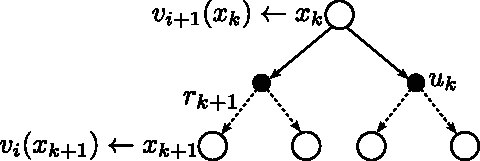
\includegraphics[width=7cm]{fig/lec03/Back_Up_Value_Policy_Evaluation.pdf}
	\caption{Backup diagram for iterative policy evaluation}
	\label{fig:Back_Up_Value_Policy_Evaluation}
\end{figure}
}


%%%%%%%%%%%%%%%%%%%%%%%%%%%%%%%%%%%%%%%%%%%%%%%%%%%%%%%%%%%%%
%% Iterative Policy Evaluation by Richardson Iteration (2)%%
%%%%%%%%%%%%%%%%%%%%%%%%%%%%%%%%%%%%%%%%%%%%%%%%%%%%%%%%%%%%%
\frame{\frametitle{Iterative Policy Evaluation by Richardson Iteration (2)}
\begin{itemize}
	\item During one Richardson iteration the 'old' value of $x_k$ is replaced with a 'new' value from the 'old' values of the successor state $x_{k+1}$.
	\begin{itemize}
		\item Update $v_{i+1}(x_k)$ from $v_{i}(x_{k+1})$, see \figref{fig:Back_Up_Value_Policy_Evaluation}.
		\item Updating estimates $(v_{i+1})$ on the basis of other estimates $(v_{i})$ is often called \hl{bootstrapping}.
	\end{itemize}\pause
	\item The Richardson iteration can be interpreted as a gradient descent algorithm for solving \eqref{eq:Bellman_matrix_Ab}.\pause
	\item This leads to \hl{synchronous, full backups} of the entire state space $\mathcal{X}$.\pause
	\item Also called \hl{expected update} because it is based on the expectation over all possible next states (utilizing full knowledge).\pause
	\item In subsequent lectures, the expected update will be supplemented by data-driven samples from the environment.
\end{itemize}

}

%%%%%%%%%%%%%%%%%%%%%%%%%%%%%%%%%%%%%%%%%%%%%%%%%%%%%%%%%%%%%
%% Iterative Policy Evaluation Example: Forest Tree MDP%%
%%%%%%%%%%%%%%%%%%%%%%%%%%%%%%%%%%%%%%%%%%%%%%%%%%%%%%%%%%%%%
\frame{\frametitle{Iterative Policy Evaluation Example: Forest Tree MDP}
Let's reuse the forest tree MDP example from \figref{fig:Forest_Markov_Decision_Process_State_Value} with \textit{fifty-fifty policy} and discount factor $\gamma=0.8$
plus disaster probability $\alpha=0.2$:
\begin{equation*}
	\bm{\mathcal{P}}_{xx'}^{\pi} = \begin{bmatrix}0 & \frac{1-\alpha}{2} & 0 & \frac{1+\alpha}{2}  \\ 0 & 0 &\frac{1-\alpha}{2} & \frac{1+\alpha}{2} \\ 0 & 0 &\frac{1-\alpha}{2} & \frac{1+\alpha}{2} \\ 0 & 0 & 0 & 1\end{bmatrix}, \quad\bm{r}_{\mathcal{X}}^{\pi} = \begin{bmatrix}0.5 \\ 1 \\ 2 \\ 0 \end{bmatrix} \, .
\end{equation*}
\pause
\begin{table}
	\centering
		\begin{tabular}{l|l|l|l|l}
			$i$ & $v_i(x=1)$ & $v_i(x=2)$ & $v_i(x=3)$ & $v_i(x=4)$\\
			\hline
			0  & 0 & 0 & 0 & 0\\ \pause
			1  & 0.5 & 1 & 2 &0\\ \pause
			2  & 0.82 & 1.64 & 2.64 & 0\\ \pause
			3  & 1.03 & 1.85 & 2.85 & 0\\ \pause
			\vdots & \vdots & \vdots & \vdots & \vdots \\
			$\infty$ & 1.12 & 1.94 & 2.94 & 0
		\end{tabular}	
	\label{tab:Forest_tree_policy_eval}
	\caption{Policy evaluation by Richardson iteration \eqref{eq:iterative_policy_eval_matrix} for forest tree MDP}
\end{table}
}

%%%%%%%%%%%%%%%%%%%%%%%%%%%%%%%%%%%%%%%%%%%%%%%%%%%%%%%%%%%%%
%% Variant: In-Place Updates %%
%%%%%%%%%%%%%%%%%%%%%%%%%%%%%%%%%%%%%%%%%%%%%%%%%%%%%%%%%%%%%
\frame{\frametitle{Variant: In-Place Updates}
Instead of applying \eqref{eq:iterative_policy_eval_matrix} to the entire vector $\bm{v}_{\mathcal{X},i+1}^{\pi}$ in 'one shot' (synchronous backup), an elementwise \hl{in-place} version of the policy evaluation can be carried out: 
\setlength{\algomargin}{0.5em}
\begin{algorithm}[H]
\SetKwInput{Input}{input} 
\SetKwInput{Output}{output}
\SetKwInput{Init}{init}
\SetKwInput{Param}{parameter}
\Input{full model of the MDP, i.e., $\left\langle\mathcal{X}, \mathcal{U}, \bm{\mathcal{P}}, \mathcal{R}, \gamma \right\rangle$ including policy $\pi$}
\Param{$\delta>0$ as accuracy termination threshold}
\Init{$v_0(x)\, \forall \, x\in\mathcal{X}$ arbitrary except $v_0(x)=0$ if $x$ is terminal}
 \Repeat{$\Delta<\delta$}{
		$\Delta \leftarrow 0 $\;
		\For{$\forall \, x_k\in\mathcal{X}$}{
			$\tilde{v}\leftarrow \hat{v}(x_k)$\;
			$\hat{v}(x_k)\leftarrow  \sum_{u_k\in\mathcal{U}}\pi(u_k|x_k)\left(\mathcal{R}^u_x + \gamma\sum_{x_{k+1}\in\mathcal{X}}p_{xx'}^u \hat{v}(x_{k+1})\right)$\;
			$\Delta \leftarrow \max\left(\Delta, |\tilde{v}-\hat{v}(x_k)|\right)$\;
		}
	}
\caption{
 Iterative policy evaluation using in-place updates (output: estimate of $\bm{v}_{\mathcal{X}}^{\pi}$)}
\label{algo:in_place_policy_update}
\end{algorithm}
}

%%%%%%%%%%%%%%%%%%%%%%%%%%%%%%%%%%%%%%%%%%%%%%%%%%%%%%%%%%%%%
%% In-Place Policy Evaluation Updates for Forest Tree MDP%%
%%%%%%%%%%%%%%%%%%%%%%%%%%%%%%%%%%%%%%%%%%%%%%%%%%%%%%%%%%%%%
\frame{\frametitle{In-Place Policy Evaluation Updates for Forest Tree MDP}
\begin{itemize}
	\item In-place algorithms allow to update states in a beneficial order. \pause
	\item May converge faster than regular Richardson iteration if state update order is chosen wisely (sweep through state space).\pause
	\item For forest tree MDP: reverse order, i.e., start with $x=4$.\pause
	\item As can be seen in \tabref{tab:Forest_tree_policy_eval_in_place} the in-place updates especially converge faster for the 'early states'.
\end{itemize}

\begin{table}
	\centering
		\begin{tabular}{l|l|l|l|l}
			$i$ & $v_i(x=1)$ & $v_i(x=2)$ & $v_i(x=3)$ & $v_i(x=4)$\\
			\hline
			0  & 0 & 0 & 0 & 0\\
			1  & 1.03 & 1.64 & 2 &0\\
			2  & 1.09 & 1.85 & 2.64 & 0\\
			3  & 1.11 & 1.91 & 2.85 & 0\\
			\vdots & \vdots & \vdots & \vdots & \vdots \\
			$\infty$ & 1.12 & 1.94 & 2.94 & 0
		\end{tabular}	
	\caption{In-place updates for forest tree MDP}
	\label{tab:Forest_tree_policy_eval_in_place}
\end{table}
}

%%%%%%%%%%%%%%%%%%%%%%%%%%%%%%%%%%%%%%%%%%%%%%%%%%%%%%%%%%%%%%%%%%
\section{Policy Improvement} 
%%%%%%%%%%%%%%%%%%%%%%%%%%%%%%%%%%%%%%%%%%%%%%%%%%%%%%%%%%%%%%%%%%
\begin{frame}
\frametitle{Table of Contents}
\tableofcontents[currentsection]
\end{frame}

%%%%%%%%%%%%%%%%%%%%%%%%%%%%%%%%%%%%%%%%%%%%%%%%%%%%%%%%%%%%%
%% General Idea on Policy Improvement%%
%%%%%%%%%%%%%%%%%%%%%%%%%%%%%%%%%%%%%%%%%%%%%%%%%%%%%%%%%%%%%
\frame{\frametitle{General Idea on Policy Improvement}
\vspace{-0.1cm}
\begin{itemize}
	\item If we know $v_{\pi}$ of a given MDP, how to improve the policy?\pause
	\item The simple idea of policy improvement is:
	\begin{itemize}
		\item Consider a new (non-policy conform) action $u\neq{\pi}(x_k)$.
		\item Follow thereafter the current policy $\pi$.
		\item Check the action-value of this 'new move'. If it is better than the 'old' value, take it.
	\end{itemize}
\end{itemize}
	\begin{equation}
	\label{eq:policy_improv_theo01}
			q_\pi(x_k,u_k)	= \E{R_{k+1} + \gamma 	v_{\pi}(X_{k+1})|X_{k}=x_{k},U_{k}=u_{k}}\,.
	\end{equation}\pause\vspace{-0.3cm}
\vspace{-0.1cm}
\begin{theo}{Policy improvement}{Policy_improvement}
If for any deterministic policy pair $\pi$ and $\pi'$
\begin{equation}
\label{eq:policy_improv_theo02}
	q_{\pi}(x,\pi'(x))\geq v_{\pi}(x) \quad \forall x\in\mathcal{X}
\end{equation}
applies, then the policy $\pi'$ must be as good as or better than $\pi$. Hence, it obtains greater or equal expected return
\begin{equation}
\label{eq:policy_improv_theo03}
	v_{\pi'}(x) \geq v_{\pi}(x) \quad \forall x\in\mathcal{X} .
\end{equation}
\end{theo}
}

%%%%%%%%%%%%%%%%%%%%%%%%%%%%%%%%%%%%%%%%%%%%%%%%%%%%%%%%%%%%%
%% Proof of Policy Improvement Theorem %%
%%%%%%%%%%%%%%%%%%%%%%%%%%%%%%%%%%%%%%%%%%%%%%%%%%%%%%%%%%%%%
\frame{\frametitle{Proof of Policy Improvement Theorem}
Start with \eqref{eq:policy_improv_theo02} and recursively reapply \eqref{eq:policy_improv_theo01}:
\begin{equation}
\hspace{-0.35cm}
	\begin{split}
		v_{\pi}(x_k) &\leq q_{\pi}(x_k,\pi'(x_k)),\\
											&= \E{R_{k+1} + \gamma 	v_{\pi}(X_{k+1})|X_{k}=x_{k},U_{k}=\pi'(x_{k})},\\
											&= \El{R_{k+1} + \gamma 	v_{\pi}(X_{k+1})|X_{k}=x_{k}}{\pi'},\\
											&\leq \El{R_{k+1} + \gamma 	q_{\pi}(x_{k+1},\pi'(x_{k+1}))|X_{k}=x_{k}}{\pi'},\\
											&= \El{R_{k+1} + \gamma 	\El{R_{k+2} + \gamma 	v_{\pi}(X_{k+2})|X_{k+1},\pi'(x_{k+1})}{\pi'}|X_{k}=x_{k}}{\pi'},\\
											&= \El{R_{k+1} + \gamma 	R_{k+2} + \gamma^2 v_{\pi}(X_{k+2})|X_{k}=x_{k}}{\pi'},\\
											&\leq \El{R_{k+1} + \gamma 	R_{k+2} + \gamma^2 R_{k+3}+ \gamma^3 v_{\pi}(X_{k+3})|X_{k}=x_{k}}{\pi'},\\
											&\hspace{0.2cm}\vdots\\
											&\leq \El{R_{k+1} + \gamma 	R_{k+2} + \gamma^2 R_{k+3}+ \gamma^3 R_{k+4}+\cdots|X_{k}=x_{k}}{\pi'},\\
											&=v_{\pi'}(x_k).
	\end{split}
\end{equation}
}

%%%%%%%%%%%%%%%%%%%%%%%%%%%%%%%%%%%%%%%%%%%%%%%%%%%%%%%%%%%%%
%% Greedy Policy Improvement (1) %%
%%%%%%%%%%%%%%%%%%%%%%%%%%%%%%%%%%%%%%%%%%%%%%%%%%%%%%%%%%%%%
\frame{\frametitle{Greedy Policy Improvement (1)}
\begin{itemize}
	\item So far, policy improvement addressed only changing the policy at a single state.\pause
	\item Now, extend this scheme to all states by selecting the best action according to $q_\pi(x_{k}, u_{k})$ in every state (\hl{greedy policy improvement}):\pause
\end{itemize}
\vspace{0.25cm}
\begin{equation}
	\begin{split}
		\pi'(x_{k})&	=\argmax_{u_k\in\mathcal{U}} q_\pi(x_{k}, u_{k}),\\
										& = \argmax_{u_k\in\mathcal{U}} \E{R_{k+1} + \gamma 	v_{\pi}(X_{k+1})|X_{k}=x_{k},U_{k}=u_{k}},\\
										& = \argmax_{u_k\in\mathcal{U}} \mathcal{R}^u_x + \gamma \sum_{x_{k+1}\in\mathcal{X}}p_{xx'}^u v_\pi(x_{k+1}) \, .
	\end{split}
\end{equation}
\begin{itemize}
	\item Again, consider that $\mathcal{R}^u_x$ could be of deterministic or stochastic nature.
\end{itemize}
}

%%%%%%%%%%%%%%%%%%%%%%%%%%%%%%%%%%%%%%%%%%%%%%%%%%%%%%%%%%%%%
%% Greedy Policy Improvement (2) %%
%%%%%%%%%%%%%%%%%%%%%%%%%%%%%%%%%%%%%%%%%%%%%%%%%%%%%%%%%%%%%
\frame{\frametitle{Greedy Policy Improvement (2)}
\begin{itemize}
	\item Each greedy policy improvement takes the best action in a one-step look-ahead search and, therefore, satisfies \theoref{theo:Policy_improvement}.\pause
	\item If after a policy improvement step $v_{\pi}(x_k) = v_{\pi'}(x_k)$ applies, it follows:
\end{itemize}
\vspace{0.25cm}
\begin{equation}
	\begin{split}
		v_{\pi'}(x_k) &=	\max_{u_k\in\mathcal{U}} \E{R_{k+1} + \gamma 	v_{\pi'}(X_{k+1})|X_{k}=x_{k},U_{k}=u_{k}},\\
										& = \max_{u_k\in\mathcal{U}} \mathcal{R}^u_x + \gamma \sum_{x_{k+1}\in\mathcal{X}}p_{xx'}^u v_{\pi'}(x_{k+1}) \, .
	\end{split}
\end{equation}\pause
\begin{itemize}
	\item This is the Bellman optimality equation, which guarantees that $\pi'=\pi$ must be optimal policies.\pause
	\item Although proof for policy improvement theorem was presented for deterministic policies, transfer to stochastic policies $\pi(u_k|x_k)$ is possible.\pause
	\item Takeaway message: \hl{policy improvement theorem guarantees finding optimal policies in finite MDPs} (e.g., by DP).
\end{itemize}	
}

%%%%%%%%%%%%%%%%%%%%%%%%%%%%%%%%%%%%%%%%%%%%%%%%%%%%%%%%%%%%%%%%%%
\section{Policy and Value Iteration} 
%%%%%%%%%%%%%%%%%%%%%%%%%%%%%%%%%%%%%%%%%%%%%%%%%%%%%%%%%%%%%%%%%%
\begin{frame}
\frametitle{Table of Contents}
\tableofcontents[currentsection]
\end{frame}

%%%%%%%%%%%%%%%%%%%%%%%%%%%%%%%%%%%%%%%%%%%%%%%%%%%%%%%%%%%%%
%% Concept of Policy Iteration %%
%%%%%%%%%%%%%%%%%%%%%%%%%%%%%%%%%%%%%%%%%%%%%%%%%%%%%%%%%%%%%
\frame{\frametitle{Concept of Policy Iteration}
\begin{itemize}
	\item Policy iteration \hl{combines the previous policy evaluation and policy improvement} in an iterative sequence: 
\end{itemize}
\vspace{0.25cm}
\begin{equation}
\label{eq:policy_iter}
	\pi_0 \rightarrow v_{\pi_0} \rightarrow \pi_1 \rightarrow v_{\pi_1} \rightarrow \cdots \pi^* \rightarrow v_{\pi^*}
\end{equation}
\begin{itemize}
	\item Evaluate $\rightarrow$ improve $\rightarrow$ evaluate $\rightarrow$ improve ...\pause
	\item In the 'classic' policy iteration, each policy evaluation step in \eqref{eq:policy_iter} is fully executed, i.e., for each policy $\pi_i$ an exact estimate of $v_{\pi_i}$ is provided either by iterative policy evaluation with a sufficiently high number of steps or by any other method that fully solves \eqref{eq:Bellman_matrix_Ab}.
\end{itemize}
}

%%%%%%%%%%%%%%%%%%%%%%%%%%%%%%%%%%%%%%%%%%%%%%%%%%%%%%%%%%%%%
%% Policy Iteration Example: Forest Tree MDP (1) %%
%%%%%%%%%%%%%%%%%%%%%%%%%%%%%%%%%%%%%%%%%%%%%%%%%%%%%%%%%%%%%
\frame{\frametitle{Policy Iteration Example: Forest Tree MDP (1)}
\begin{figure}		
	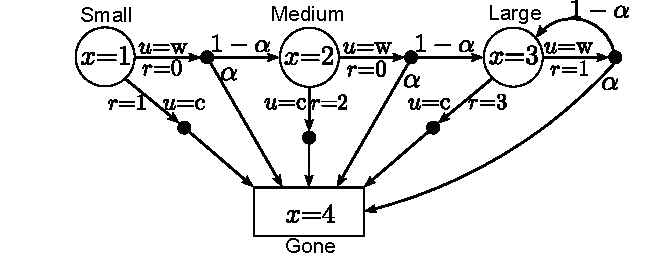
\includegraphics[width=11cm]{fig/lec03/Forest_Markov_Decision_Process.pdf}
\end{figure}
\begin{itemize}
	\item Two actions possible in each state:
	\begin{itemize}
		\item Wait $u=w$: let the tree grow.
		\item Cut $u=c$: gather the wood.
	\end{itemize}
\end{itemize}
}

%%%%%%%%%%%%%%%%%%%%%%%%%%%%%%%%%%%%%%%%%%%%%%%%%%%%%%%%%%%%%
%% Policy Iteration Example: Forest Tree MDP (2) %%
%%%%%%%%%%%%%%%%%%%%%%%%%%%%%%%%%%%%%%%%%%%%%%%%%%%%%%%%%%%%%
\frame{\frametitle{Policy Iteration Example: Forest Tree MDP (2)}
Assume $\alpha=0.2$ and $\gamma=0.8$ and start with \hl{'tree hater' initial policy}:\pause
\begin{enumerate}
	\item $\pi_0=\pi(u_k =\mbox{c}|x_k) \quad \,\forall x_k\in\mathcal{X}$.\pause
	\item Policy evaluation: $v_\mathcal{X}^{\pi_0}=\begin{bmatrix}1 & 2 & 3 & 0\end{bmatrix}^T$\pause
	\item Greedy policy improvement: 
	\begin{equation*}
	\begin{split}
		\pi_1(x_{k})& = \argmax_{u_k\in\mathcal{U}} \E{R_{k+1} + \gamma 	v_{\pi_0}(X_{k+1})|X_{k}=x_{k},U_{k}=u_{k}},\\
										& = \left\{\pi(u_k =\mbox{w}|x_k=1), \pi(u_k =\mbox{c}|x_k=2), \pi(u_k =\mbox{c}|x_k=3)\right\}
	\end{split}
\end{equation*}\pause
\item Policy evaluation: $v_\mathcal{X}^{\pi_1}=\begin{bmatrix}1.28 & 2 & 3 & 0\end{bmatrix}^T$\pause
\item Greedy policy improvement: 
	\begin{equation*}
	\begin{split}
		\pi_2(x_{k})& = \argmax_{u_k\in\mathcal{U}} \E{R_{k+1} + \gamma 	v_{\pi_1}(X_{k+1})|X_{k}=x_{k},U_{k}=u_{k}},\\
										& = \left\{\pi(u_k =\mbox{w}|x_k=1), \pi(u_k =\mbox{c}|x_k=2), \pi(u_k =\mbox{c}|x_k=3)\right\},\\
										& = \pi_1(x_{k})\\
										& = \pi^*
	\end{split}
\end{equation*}
\end{enumerate}
}

%%%%%%%%%%%%%%%%%%%%%%%%%%%%%%%%%%%%%%%%%%%%%%%%%%%%%%%%%%%%%
%% Policy Iteration Example: Forest Tree MDP (3) %%
%%%%%%%%%%%%%%%%%%%%%%%%%%%%%%%%%%%%%%%%%%%%%%%%%%%%%%%%%%%%%
\frame{\frametitle{Policy Iteration Example: Forest Tree MDP (3)}
Assume $\alpha=0.2$ and $\gamma=0.8$ and start with \hl{'tree lover' initial policy}:\pause
\begin{enumerate}
	\item $\pi_0=\pi(u_k =\mbox{w}|x_k) \quad \,\forall x_k\in\mathcal{X}$.\pause
	\item Policy evaluation: $v_\mathcal{X}^{\pi_0}=\begin{bmatrix}1.14 & 1.78 & 2.78 & 0\end{bmatrix}^T$\pause
	\item Greedy policy improvement: 
	\begin{equation*}
	\begin{split}
		\pi_1(x_{k})& = \argmax_{u_k\in\mathcal{U}} \E{R_{k+1} + \gamma 	v_{\pi_0}(X_{k+1})|X_{k}=x_{k},U_{k}=u_{k}},\\
										& = \left\{\pi(u_k =\mbox{w}|x_k=1), \pi(u_k =\mbox{c}|x_k=2), \pi(u_k =\mbox{c}|x_k=3)\right\}
	\end{split}
\end{equation*}\pause
\item Policy evaluation: $v_\mathcal{X}^{\pi_1}=\begin{bmatrix}1.28 & 2 & 3 & 0\end{bmatrix}^T$\pause
\item Greedy policy improvement: 
	\begin{equation*}
	\begin{split}
		\pi_2(x_{k})& = \argmax_{u_k\in\mathcal{U}} \E{R_{k+1} + \gamma 	v_{\pi_1}(X_{k+1})|X_{k}=x_{k},U_{k}=u_{k}},\\
										& = \left\{\pi(u_k =\mbox{w}|x_k=1), \pi(u_k =\mbox{c}|x_k=2), \pi(u_k =\mbox{c}|x_k=3)\right\},\\
										& = \pi_1(x_{k})\\
										& = \pi^*
	\end{split}
\end{equation*}
\end{enumerate}
}

%%%%%%%%%%%%%%%%%%%%%%%%%%%%%%%%%%%%%%%%%%%%%%%%%%%%%%%%%%%%%
%% Policy Iteration Example: Jack's Car Rental (1) %%
%%%%%%%%%%%%%%%%%%%%%%%%%%%%%%%%%%%%%%%%%%%%%%%%%%%%%%%%%%%%%
\frame{\frametitle{Policy Iteration Example: Jack's Car Rental (1)}
\begin{figure}		
	
\includegraphics[width=2cm]{fig/lec03/car_rental.pdf}
\end{figure}
\begin{itemize}
	\item States: Two rental locations, maximum of 20 cars each\pause
	\item Actions: Move up to 5 cars between locations overnight\pause
	\item Reward: 
	\begin{itemize}
		\item  +10 \$ for each car rented (if available at location)
		\item -2 \$ for each overnight car transfer
		\item Discount: $\gamma=0.9$
	\end{itemize}\pause 
	\item Dynamics: Cars returned and requested randomly following Poisson distribution
	\begin{itemize}
		\item $P_\lambda(n)=\frac{\lambda^n}{n!}e^{-\lambda}$
		\item $P_\lambda(n)=$ probability of observing $n$ events with mean event rate $\lambda$
		\item 1st location: $\lambda_{\mbox{req.}}=3$, $\lambda_{\mbox{ret.}}=3$
		\item 2nd location: $\lambda_{\mbox{req.}}=4$, $\lambda_{\mbox{ret.}}=2$
	\end{itemize}
\end{itemize}
}

%%%%%%%%%%%%%%%%%%%%%%%%%%%%%%%%%%%%%%%%%%%%%%%%%%%%%%%%%%%%%
%% Policy Iteration Example: Jack's Car Rental (2) %%
%%%%%%%%%%%%%%%%%%%%%%%%%%%%%%%%%%%%%%%%%%%%%%%%%%%%%%%%%%%%%
\frame{\frametitle{Policy Iteration Example: Jack's Car Rental (2)}
\begin{figure}
		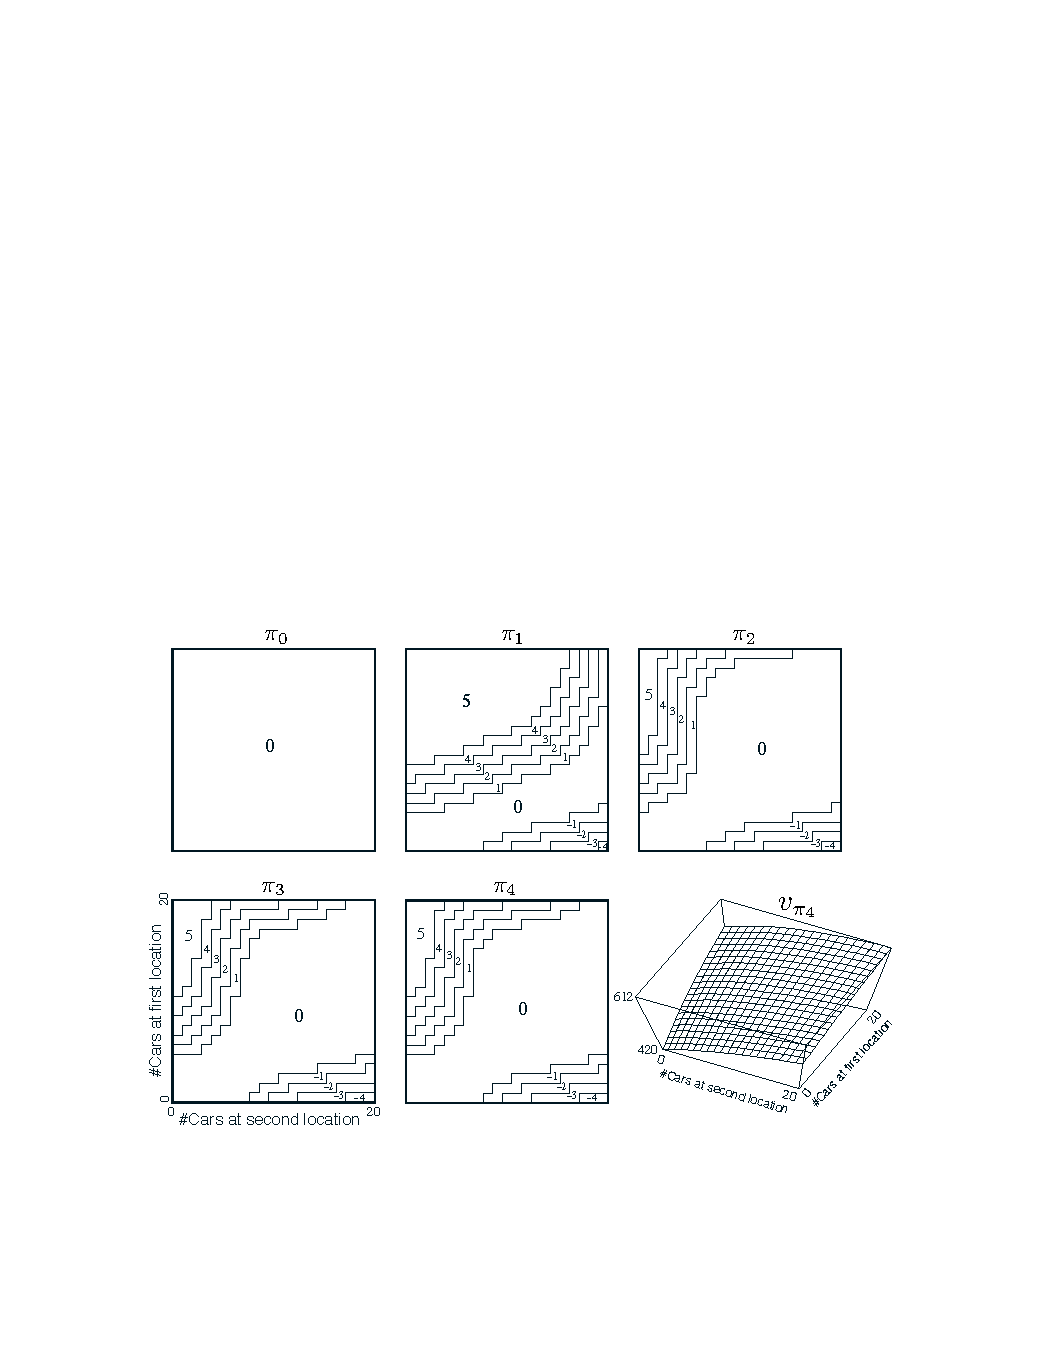
\includegraphics[width=9cm]{fig/lec03/Jack_Car_Rental.pdf}
		\caption{Sequence of policies found by policy iteration including optimal state value after termination (source: R. Sutton and G. Barto, Reinforcement learning: an introduction, 2018, \href{https://creativecommons.org/licenses/by-nc-nd/2.0/}{CC BY-NC-ND 2.0})}
		\label{fig:Jack_Car_Rental}
	\end{figure}
}

%%%%%%%%%%%%%%%%%%%%%%%%%%%%%%%%%%%%%%%%%%%%%%%%%%%%%%%%%%%%%
%% Value Iteration (1) %%
%%%%%%%%%%%%%%%%%%%%%%%%%%%%%%%%%%%%%%%%%%%%%%%%%%%%%%%%%%%%%
\frame{\frametitle{Value Iteration (1)}
\begin{itemize}
	\item Policy iteration involves full policy evaluation steps between policy improvements.
	\item In large state-space MDPs the full policy evaluation may be numerically very costly.\pause
	\item Using a limited number of iterative policy evaluations steps and then apply policy improvement may speed up the entire DP process.\pause
	\item \hl{Value iteration}: One step iterative policy evaluation followed by policy improvement.\pause
	\item Allows simple update rule which \hl{combines policy improvement with truncated policy evaluation}:
	\begin{equation}
	\begin{split}
		v_{i+1}(x_k) &=	\max_{u_k\in\mathcal{U}} \E{R_{k+1} + \gamma 	v_{i}(X_{k+1})|X_{k}=x_{k},U_{k}=u_{k}},\\
										&= \max_{u_k\in\mathcal{U}} \mathcal{R}^u_x + \gamma \sum_{x_{k+1}\in\mathcal{X}}p_{xx'}^u v_{i}(x_{k+1}) \, .
	\end{split}
\end{equation}
\end{itemize}
}

%%%%%%%%%%%%%%%%%%%%%%%%%%%%%%%%%%%%%%%%%%%%%%%%%%%%%%%%%%%%%
%% Value Iteration (2) %%
%%%%%%%%%%%%%%%%%%%%%%%%%%%%%%%%%%%%%%%%%%%%%%%%%%%%%%%%%%%%%
\frame{\frametitle{Value Iteration (2)}
\setlength{\algomargin}{0.5em}
\begin{algorithm}[H]
\SetKwInput{Input}{input} 
\SetKwInput{Output}{output}
\SetKwInput{Init}{init}
\SetKwInput{Param}{parameter}
\Input{full model of the MDP, i.e., $\left\langle\mathcal{X}, \mathcal{U}, \bm{\mathcal{P}}, \mathcal{R}, \gamma \right\rangle$}
\Param{$\delta>0$ as accuracy termination threshold}
\Init{$v_0(x)\, \forall \, x\in\mathcal{X}$ arbitrary except $v_0(x)=0$ if $x$ is terminal}
 \Repeat{$\Delta<\delta$}{
		$\Delta \leftarrow 0 $\;
		\For{$\forall \, x_k\in\mathcal{X}$}{
			$\tilde{v}\leftarrow \hat{v}(x_k)$\;
			$\hat{v}(x_k)\leftarrow  \max_{u_k\in\mathcal{U}}\left(\mathcal{R}^u_x + \gamma\sum_{x_{k+1}\in\mathcal{X}}p_{xx'}^u \hat{v}(x_{k+1})\right)$\;
			$\Delta \leftarrow \max\left(\Delta, |\tilde{v}-\hat{v}(x_k)|\right)$\;
		}
	}
\Output{Deterministic policy $\pi\approx\pi^*$, such that}
	$\pi(x_k)\leftarrow  \argmax_{u_k\in\mathcal{U}}\left(\mathcal{R}^u_x + \gamma\sum_{x_{k+1}\in\mathcal{X}}p_{xx'}^u \hat{v}(x_{k+1})\right)$\;
\caption{Value iteration (note: compared to policy iteration, value iteration doesn't require an initial policy but only a state-value guess)}
\end{algorithm}
}

%%%%%%%%%%%%%%%%%%%%%%%%%%%%%%%%%%%%%%%%%%%%%%%%%%%%%%%%%%%%%
%% Value Iteration for Forest Tree MDP %%
%%%%%%%%%%%%%%%%%%%%%%%%%%%%%%%%%%%%%%%%%%%%%%%%%%%%%%%%%%%%%
\frame{\frametitle{Value Iteration for Forest Tree MDP}
\begin{figure}		
	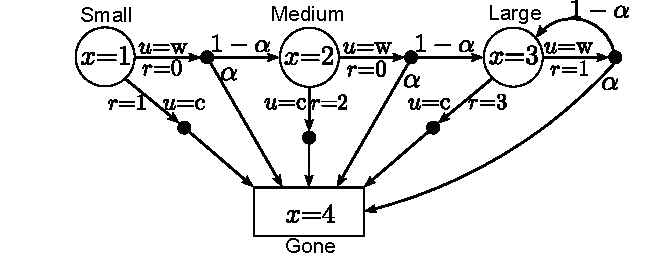
\includegraphics[width=6cm]{fig/lec03/Forest_Markov_Decision_Process.pdf}
\end{figure}
\begin{itemize}
	\item Assume again $\alpha=0.2$ and $\gamma=0.8$.\pause
	\item Similar to in-place update policy evaluation, reverse order and start value iteration with $x=4$.\pause
	\item As shown in \tabref{tab:Forest_tree_value_iteration} value iteration converges in one step (for the given problem) to the optimal state-value. 
\end{itemize}
\begin{table}
	\centering
		\begin{tabular}{l|l|l|l|l}
			$i$ & $v_i(x=1)$ & $v_i(x=2)$ & $v_i(x=3)$ & $v_i(x=4)$\\
			\hline
			0  & 0 & 0 & 0 & 0\\
			1  & 1.28 & 2 & 3 &0\\
			*  & 1.28 & 2 & 3 &0
		\end{tabular}	
	\caption{Value iteration for forest tree MDP}
	\label{tab:Forest_tree_value_iteration}
\end{table}
}


%%%%%%%%%%%%%%%%%%%%%%%%%%%%%%%%%%%%%%%%%%%%%%%%%%%%%%%%%%%%%%%%%%
\section{Further Aspects} 
%%%%%%%%%%%%%%%%%%%%%%%%%%%%%%%%%%%%%%%%%%%%%%%%%%%%%%%%%%%%%%%%%%
\begin{frame}
\frametitle{Table of Contents}
\tableofcontents[currentsection]
\end{frame}

%%%%%%%%%%%%%%%%%%%%%%%%%%%%%%%%%%%%%%%%%%%%%%%%%%%%%%%%%%%%%
%% Summarizing DP Algorithms %%
%%%%%%%%%%%%%%%%%%%%%%%%%%%%%%%%%%%%%%%%%%%%%%%%%%%%%%%%%%%%%
\frame{\frametitle{Summarizing DP Algorithms}
\begin{itemize}
	\item All DP algorithms are based on the state-value $v(x)$.
	\begin{itemize}
		\item Complexity is $\mathcal{O}(m\cdot n^2)$ for $m$ actions and $n$ states.
		\item Evaluate all $n^2$ state transitions while considering up to $m$ actions per state.
	\end{itemize}\pause
	\item Could be also applied to action-values $q(x,u)$.
	\begin{itemize}
		\item Complexity is inferior with $\mathcal{O}(m^2\cdot n^2)$.
		\item There are up to $m^2$ action-values which require $n^2$ state transition evaluations each.
	\end{itemize}
\end{itemize}
\pause
\begin{table}
	\centering
		\begin{tabular}{|M{1.65cm}||M{4.75cm}|M{4cm}|}
			\hline
			Problem & Relevant Equations & Algorithm\\
			\hline\hline
			prediction & Bellman expectation eq. &  policy evaluation\\
			\hline
			control & Bellman expectation eq. \& greedy policy improvement & policy iteration\\
			\hline
			control & Bellman optimality eq. & value iteration\\
			\hline
		\end{tabular}	
		\caption{Short overview addressing the treated DP algorithms}
		\label{tab:DP_syn_algos}
\end{table}
}

%%%%%%%%%%%%%%%%%%%%%%%%%%%%%%%%%%%%%%%%%%%%%%%%%%%%%%%%%%%%%
%%Asynchronous DP%%
%%%%%%%%%%%%%%%%%%%%%%%%%%%%%%%%%%%%%%%%%%%%%%%%%%%%%%%%%%%%%
\frame{\frametitle{Asynchronous DP}
\begin{itemize}
	\item DP algorithms considered so far used \hl{synchronous backups}:
	\begin{itemize}
		\item In one iteration the entire state space is updated.
		\item May be computational expensive for large MDPs.
		\item Some state-values or policy parts may converge faster than other but are updated as often as slowly converging states.
	\end{itemize}
	\vspace{0.5cm}\pause
	\item In contrast, \hl{asynchronous backups} update states individually in an (arbitrary) order:
	\begin{itemize}
		\item Choose smart order to achieve faster overall convergence rate.
		\item Some states may be updated more frequently than others.\pause
		\item Overall algorithms converges if all states are still visited to some extent (\hl{important requirement to ensure convergence}).\pause
		\item Simple example: in-place policy evaluation where only a subset of all states are updated each iterations (cf. \algoref{algo:in_place_policy_update}).
	\end{itemize}
\end{itemize}
}

%%%%%%%%%%%%%%%%%%%%%%%%%%%%%%%%%%%%%%%%%%%%%%%%%%%%%%%%%%%%%
%% Asynchronous DP: Prioritized Sweeping %%
%%%%%%%%%%%%%%%%%%%%%%%%%%%%%%%%%%%%%%%%%%%%%%%%%%%%%%%%%%%%%
\frame{\frametitle{Asynchronous DP: Prioritized Sweeping}
\begin{itemize}
	\item Use magnitude of \hl{Bellman error} as an indicator which state should be updated next:
	\begin{equation}
		\argmax_{x_k\in\mathcal{X}}\left|\max_{u_k\in\mathcal{U}} \left(\mathcal{R}^u_x + \gamma \sum_{x_{k+1}\in\mathcal{X}}p_{xx'}^u v_{i}(x_{k+1})\right) - v_i(x_k)\right|\, .
	\end{equation}\pause
	\item Update the state with the largest Bellman error first. 
	\item Build up a priority queue of most relevant states by refreshing the Bellman error after each state update.
\end{itemize}
}

%%%%%%%%%%%%%%%%%%%%%%%%%%%%%%%%%%%%%%%%%%%%%%%%%%%%%%%%%%%%%
%% Asynchronous DP: Real-Time Updates %%
%%%%%%%%%%%%%%%%%%%%%%%%%%%%%%%%%%%%%%%%%%%%%%%%%%%%%%%%%%%%%
\frame{\frametitle{Asynchronous DP: Real-Time Updates}
\begin{itemize}
	\item Update those states which are frequently visited by the agent.
	\item Utilizes agent's experience to guide the asynchronous DP updates.
	\item After each time step $\left\langle x_k, u_k, r_{k+1}\right\rangle$ update $x_k$:
	\begin{equation}
		v_i(x_k) \leftarrow \max_{u_k\in\mathcal{U}} \left(\mathcal{R}^u_{x} + \gamma \sum_{x_{k+1}\in\mathcal{X}}p_{xx'}^u v_{i}(x_{k+1})\right).
	\end{equation}
\end{itemize}
\begin{figure}
		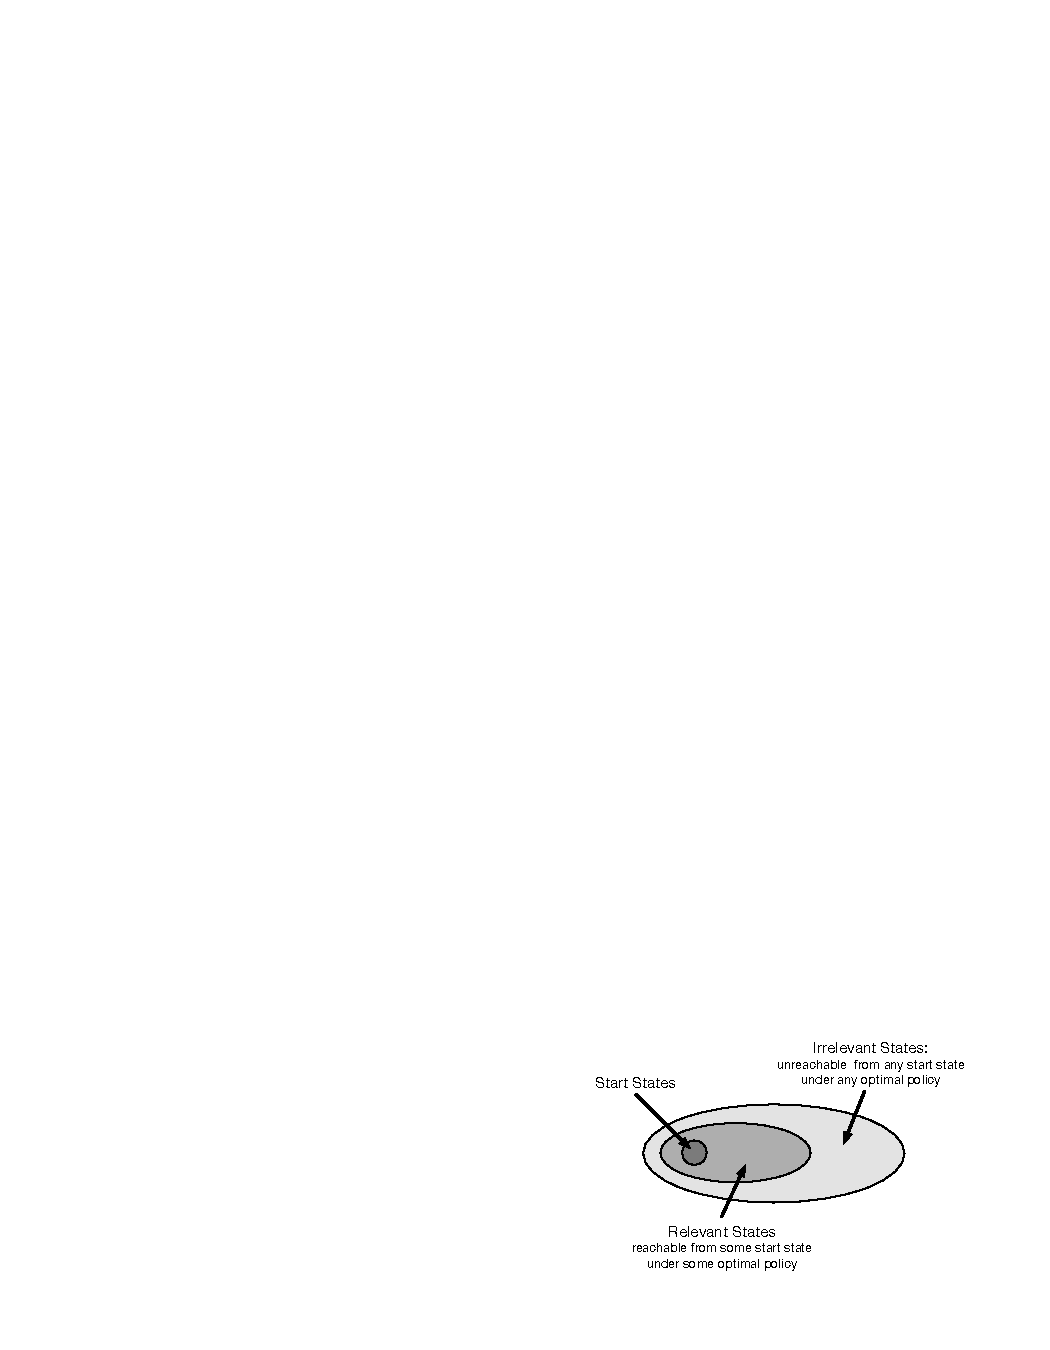
\includegraphics[width=5.5cm]{fig/lec03/RTDP.pdf}
		\caption{Real-time DP updates focus on reachable states (source: R. Sutton and G. Barto, Reinforcement learning: an introduction, 2018, \href{https://creativecommons.org/licenses/by-nc-nd/2.0/}{CC BY-NC-ND 2.0})}
		\label{fig:RTDP}
\end{figure}
}

%%%%%%%%%%%%%%%%%%%%%%%%%%%%%%%%%%%%%%%%%%%%%%%%%%%%%%%%%%%%%
%% Generalized Policy Iteration %%
%%%%%%%%%%%%%%%%%%%%%%%%%%%%%%%%%%%%%%%%%%%%%%%%%%%%%%%%%%%%%
\frame{\frametitle{Generalized Policy Iteration (GPI)}
\begin{itemize}
	\item Almost all RL methods are well-described as GPI.
	\item \hl{Push-pull}: Improving the policy will deteriorate value estimation.  
	\item Well balanced \hl{trade-off between evaluating and improving} is required.
\end{itemize}
\begin{figure}
	\subfloat{
		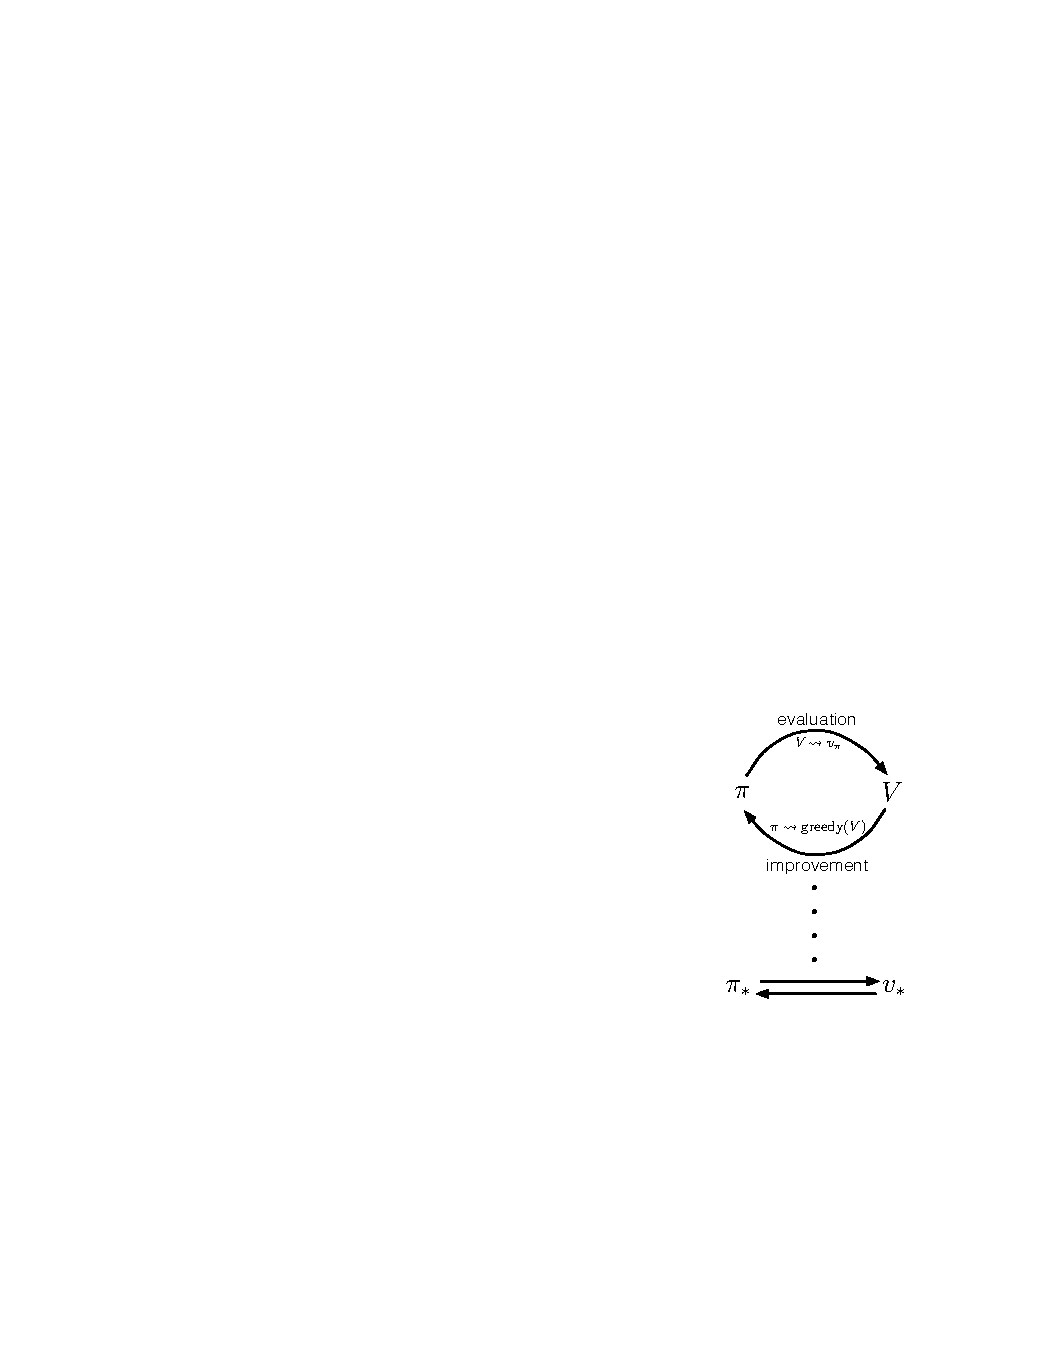
\includegraphics[height=4cm]{fig/lec03/GPI_01.pdf}
	}
	\hspace{1cm}
	\subfloat{
		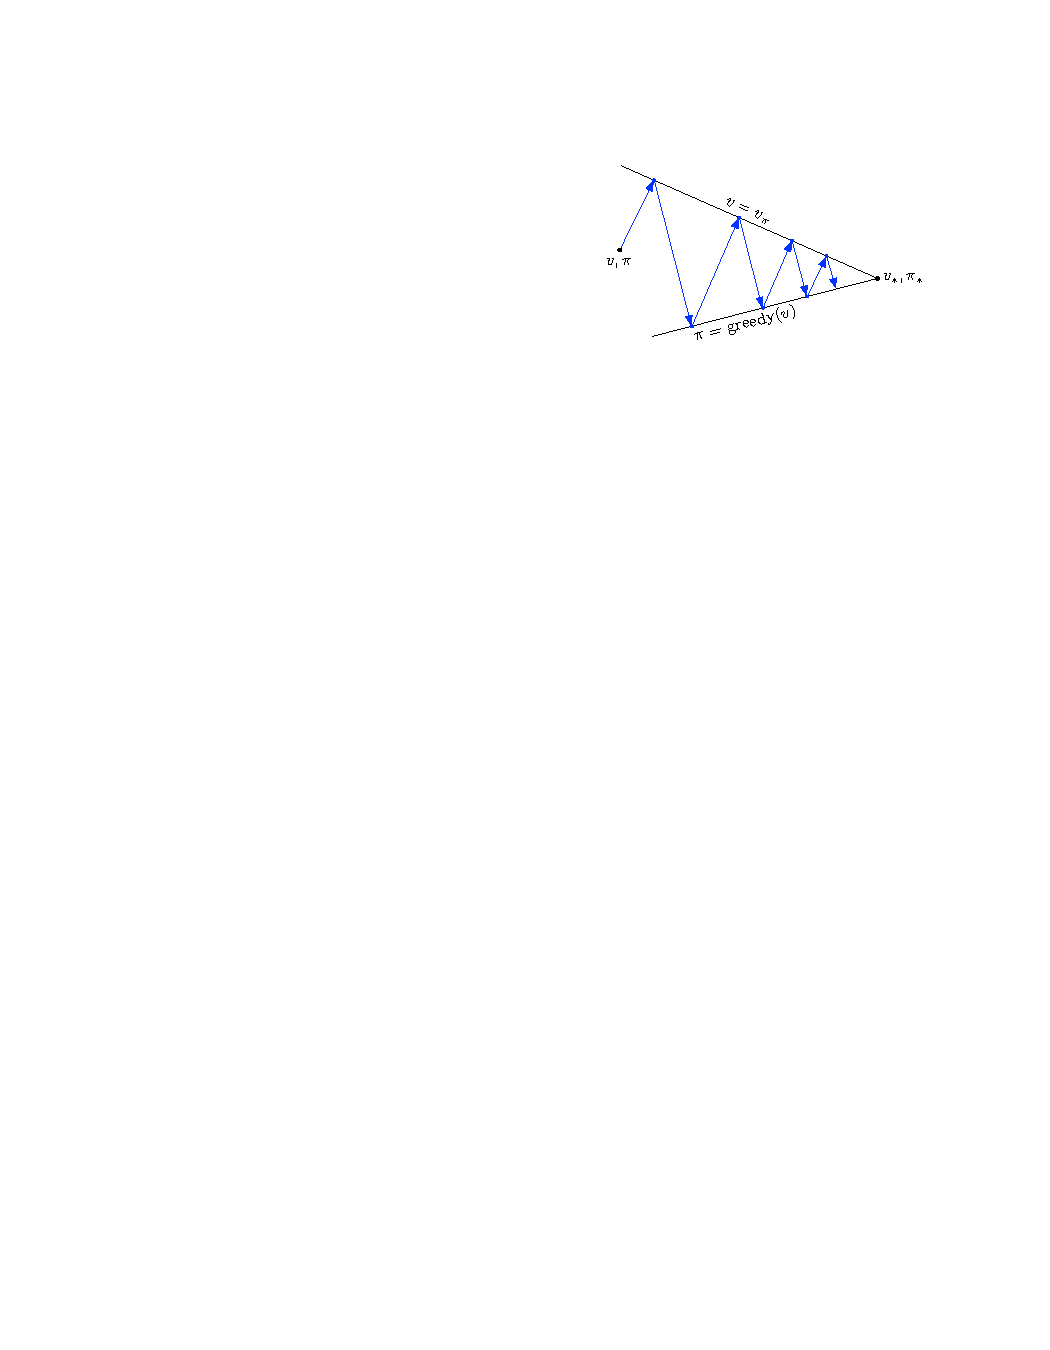
\includegraphics[height=4cm]{fig/lec03/GPI_02.pdf}
	}
\caption{Interpreting generalized policy iteration to switch back and forth between (arbitrary) evaluations and improvement steps (source: R. Sutton and G. Barto, Reinforcement learning: an introduction, 2018, \href{https://creativecommons.org/licenses/by-nc-nd/2.0/}{CC BY-NC-ND 2.0})}
\end{figure}
}

%%%%%%%%%%%%%%%%%%%%%%%%%%%%%%%%%%%%%%%%%%%%%%%%%%%%%%%%%%%%%
%% Curse of Dimensionality %%
%%%%%%%%%%%%%%%%%%%%%%%%%%%%%%%%%%%%%%%%%%%%%%%%%%%%%%%%%%%%%
\frame{\frametitle{Curse of Dimensionality}
\begin{itemize}
	\item DP is much more efficient than an exhaustive search over all $n$ states and $m$ actions in finite MDPs in order to find an optimal policy.
	\begin{itemize}
		\item Exhaustive search for deterministic policies: $m^n$ evaluations.
		\item DP results in polynomial complexity regarding $m$ and $n$. 
	\end{itemize}
	\pause
	\item Nevertheless, DP uses full-width backups:
	\begin{itemize}
		\item For each state update, every successor state and action is considered.
		\item While utilizing full knowledge of the MDP structure.
	\end{itemize}
	\pause
	\item Hence, DP is can be effective up to medium-sized MDPs (i.e., million states)\pause
	\item For large problems DP suffers from the \hl{curse of dimensionality}:
	\begin{itemize}
		\item Number of finite states $n$ grows exponentially with the number of state variables.
		\item Also: if continuous variables need quantization typically a large number of states results. 
		\item Single state update may become computational infeasible. 
	\end{itemize}
\end{itemize}
}

%%%%%%%%%%%%%%%%%%%%%%%%%%%%%%%%%%%%%%%%%%%%%%%%%%%%%%%%%%%%%
%% Summary %%
%%%%%%%%%%%%%%%%%%%%%%%%%%%%%%%%%%%%%%%%%%%%%%%%%%%%%%%%%%%%%
\begin{frame}
\frametitle{Summary: What You've Learned Today}
\begin{itemize}
	\item DP is applicable for prediction and control problems in MDPs.\pause
	\item But requires always full knowledge about the environment (i.e., it is a model-based solution also called planning).\pause
	\item DP is more efficient than exhaustive search.\pause
	\item But suffers from the curse of dimensionality for large MDPs.\pause
	\item (Iterative) policy evaluations and (greedy) improvements solve MDPs.\pause
	\item Both steps can be combined via value iteration.\pause
	\item This idea of (generalized) policy iteration is a basic scheme of RL.\pause
	\item Implementing DP algorithms comes with many degrees of freedom.
	\item For example how to order the state updates (asyn. vs. sync.).
\end{itemize}
\end{frame}

%%%%%%%%%%%%%%%%%%%%%%%%%%%%%%%%%%%%%%%%%%%%%%%%%%%%%%%%%%%%%
%% Final Slide %%
%%%%%%%%%%%%%%%%%%%%%%%%%%%%%%%%%%%%%%%%%%%%%%%%%%%%%%%%%%%%%
\frame{\frametitle{The End for Today}
\begin{figure}

\includegraphics[width=10cm]{fig/lec03/dilbert.jpg}
\end{figure}
\vspace{1cm}
\centering
Thanks for your attention and have a nice week!
}
